\documentclass{standalone}
\usepackage{tikz}
\usepackage{lmodern}
\usepackage[T1]{fontenc}
\begin{document}
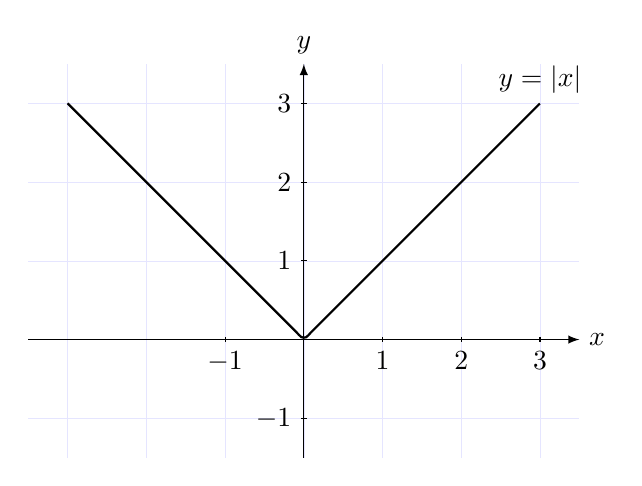
\begin{tikzpicture}[domain=-2:2,samples=100,scale=1.0,>=latex]
\tikzset{bgrid/.style={help lines,color=blue!10,very thin}}

\draw[bgrid] (-3.5,-1.5) grid (3.5,3.5);

\draw[->, color=black] (-3.5,0) -- (3.5,0) node[right] {$x$};
\draw[->, color=black] (0,-1.5) -- (0,3.5) node[above] {$y$};

\foreach \x/\xtext in {-1,1,2,3}
\draw (\x cm,1pt) -- (\x cm,-1pt) node[anchor=north] {$\xtext$};

\foreach \y/\ytext in {-1,1,2,3}
\draw (1pt,\y cm) -- (-1pt,\y cm) node[anchor=east] {$\ytext$};

\draw[thick,color=black,domain=-3:3,smooth]
plot (\x,{abs(\x)}) node[anchor=south] {$y = \left|x\right|$};
% \draw[dashed,color=black,domain=0:7.5,smooth]
% plot (\x,{(-1)*(sqrt(\x))}) node[anchor=north] {$y = -\sqrt{x}$};
% \draw[thick,color=black,domain=-1.5:5.5,samples=3]
% plot (\x,{(\x)-2}) node[anchor=south] {$y = x - 2$};

% \filldraw[black] (4,2) circle(2pt) node[anchor=south east] {$(4, 2)$};
% \filldraw[red] (1,-1) circle(2pt);
% \draw[red] (1.5,-1) node[anchor=west] {$(1, -1)$};

\end{tikzpicture}
\end{document}